\chapter{LLVM}
\section{History}
The \llvm is a collection of modular and reusable compiler and toolchain technologies to support static and dynamic compilation as well as transparent and lifelong program analysis and transformations of arbitrary programs. \cite{LLVMWebsite, LLVMResearchBeginning}\\
The main goal of \llvm consists of the creation of a compiler framework in which the optimizations and analysis are independent from the underlying OS and the used programming language.
To archive the independency \llvmir was introduced which is solely used within the pipeline.
\enquote{\llvmir is a strongly typed, \ac{SSA} language that connects to a wide variety of high-level languages.} \cite{PolyhedralEmpiricalStudy}\\
Originally \llvm has been a reasearch project, which was first described in a publication in 2004, at the university of Illinois.
Since that the project has grown so popular that in 2014 the LLVM Foundation was founded for organizing and maintaining the project. \cite{LLVMFoundation}\\

\section{Pipeline}
When entering the pipeline of \llvm (\autoref{fig:llvmPipeline}) the \llvmir putting the independence from the programing language into effect is generated by translating the files containing sourcecode written in an arbitrary programming language using a frontend like clang.
When leaving the pipeline files containing the appropriate assembler instructions are created out of the (possibly) newly formed \llvmir. \cite{IntroLLVM}
\begin{figure}[!ht]
    \caption{A possible pipeline of LLVM}
    \label{fig:llvmPipeline}
    \centering
    \begin{tikzlegend}
        \node(languages)[nonLlvmIrNode, align=center]{C/C++, Obj-C,\\Python, Ruby,...};
        \node(frontend)[nonLlvmIrNode, right=of languages]{compiler frontend};
        \node(opt1)[llvmIrNode, right=of frontend]{\opt};
        \node(llvmLinker)[llvmIrNode, below=of opt1]{\linker};
        \node(opt2)[llvmIrNode, below=of llvmLinker]{\opt};
        \node(generator)[llvmIrNode, left=of opt2]{\generator};
        \node(linker)[nonLlvmIrNode, left=of generator]{System Linker};
        \path[nonLlvmIrPath] (languages) to (frontend);
        \path[llvmIrPath] (frontend) to (opt1);
        \path[llvmIrPath] (opt1) -| ($(opt1.north east) + (0.5,0.5)$) -| node[auto]{Pass} (opt1);
        \path[llvmIrPath] (opt2) -| ($(opt2.south east) + (0.5,-0.5)$) -| node[auto]{Pass} (opt2);
        \path[llvmIrPath] (opt1) to node[auto, swap]{Multiple files} (llvmLinker);
        \path[llvmIrPath] (llvmLinker) to node[auto, swap]{Single file} (opt2);
        \path[llvmIrPath] (opt2) to (generator);
        \path[nonLlvmIrPath] (generator) to (linker);
    \end{tikzlegend}
\end{figure}\\
\subsection{compiler frontend}\label{subsec:compilerfrontend}
The first step of the pipeline is translating the files containing sourcecode by a front end like clang (C, C++, Objective-C), llvm-gfortran (Fortran), PyLLVM (Python) \draftnote{cite?}, llvmRuby (Ruby) \draftnote{Still existing?}, IcedTea (Java) or .NET \draftnote{cite GrosserDiploma}.
From now on this work is only discussing clang as frontend.
This study is working on C/C++ so only clang is used.
Using clang \llvmir can be generated by adding the option \texttt{-emit-llvm} in order \enquote{to abstract away from the specifics} \cite{FastScopDetection} of a programming language.
The option \texttt{-S} may also be passed to generate a human readable textfile instead of a \llvmir binary.
\subsection{LLVM Optimizer}\label{subsec:optimizer}
On files containing \llvmir the \opt can perform steps for optimizing and analysing the code.
These steps are called \enquote{Passes}.
Such passes can be invoked explicitly by appending the appropriate options to the command \texttt{opt} of the the \opt and are applied either to single files or to the already linked program.
It is also possible to add further custom options by loading (multiple) libraries using the flag \texttt{-load}.
When calling the \opt the option \texttt{-S} may also be specified for generating a human readable textfile similar to clang in \autoref{subsec:compilerfrontend}.
\subsection{LLVM Linker}
The \linker is an optional step which is taken if \draftnote{When?}.
The \linker links the optimized \llvmir files into a single \llvmir file and applies further optimizations.
\subsection{LLVM Code Generator}
When all desired passes are performed the \generator translates \llvmir into target assembler.
\subsection{Basic Blocks}
The underlying structure the pipeline is working on are \enquote{basic blocks}.
In \cite[chapter 8.4, p.~525]{Drachenbuch} basic blocks
\begin{comment}
    Seite 525, Chapter 8. Code Generation, 8.4 Basic Blocks and Flow Graphs
\end{comment}
\begin{quote}
    [...] are maximal sequences of consecutive three-address instructions with the properties that
    \begin{enumerate}[label=(\alph*)]
        \item The flow of control can only enter the basic block through the first instruction in the block.
        \item Control will leave the block without halting or branching, except possibly at the last instruction in the block.
    \end{enumerate}
\end{quote}
\subsection{Control Flow Graph (CFG)}\label{subsec:cfg}
\begin{wrapfigure}{I}{.3\textwidth}
    \caption{The CFG of \autoref{lst:matmulll}}
    \label{fig:exampleCfg}
    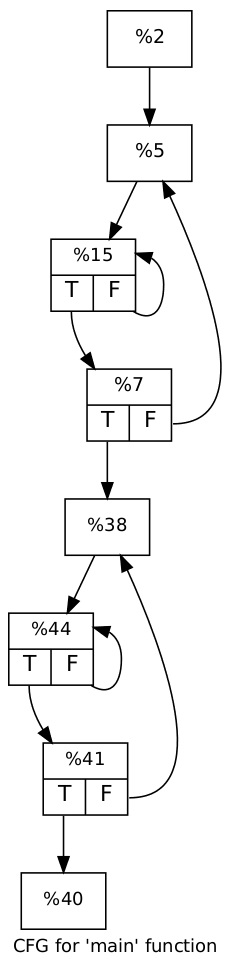
\includegraphics[height=12cm]{gfx/matmulCfg.png}
\end{wrapfigure}
The \cfg is a representation of the the control flow (connections between basic blocks) \cite[chapter 8.4.3, p.~529]{Drachenbuch}.
\begin{comment}
    Seite 529, Chapter 8. Code Generation, 8.4.3 Flow Graphs
\end{comment}
\begin{quote}
    The nodes of the flow graph are the basic blocks.
    There is an edge from block \(B\) to block \(C\) if and only if it is possible for the first instruction in block \(C\) to immediately follow the last instruction in block \(B\).
    There are two ways that such an edge could be justified:
    \begin{itemize}
        \item There is a conditio nal or unconditional jump from the end of \(B\) to the beginning of \(C\).
        \item \(C\) immediately follows \(B\) in the original ordera of the three-address instructions, and \(B\) does not end in an unconditional jump.
    \end{itemize}
\end{quote}
Therefore the \cfg is very important to the pipeline as it is needed by many analysis passes and by optimization passes to determine whether certain optimizations can be applied and which way.
The current \cfg of a \llvmir file can be generated at any point of the pipeline.
It also can be visualized (like \autoref{fig:exampleCfg}) by passing one of the options \texttt{-view-cfg} or \texttt{-view-cfg-only} to the \opt.
